\chapter{L’apprentissage automatique}
\label{chapter4}
Dans le domaine de l'intelligence artificielle, on dit qu'un agent apprend quand ses performances s’améliorent après quelques observations sur le monde. Lorsque l’agent est une machine, on appelle les observations « \textbf{data} » ou données en français et le processus « apprentissage automatique » ou apprentissage machine.

Dans l'apprentissage automatique, un ordinateur observe certaines données, construit un modèle basé sur ces données et utilise le modèle à la fois comme hypothèse sur le monde et comme logiciel capable de résoudre des problèmes (\cite{RussellNorvig2020}). Le machine learning désigne donc une famille de techniques et d’algorithmes d’apprentissage basés sur l’induction\footnote{L’induction est l’opposé de la déduction. La déduction consiste à tirer des conclusions spécifiques à partir de prémisses « générales » attestées, les conclusions tirées de la déduction sont garanties comme vraies tandis que l'induction vise à développer des conclusions générales à partir d'exemples spécifiques et peut donc conduire à des conclusions incorrectes.} utilisés pour que les machines puisse extraire des « connaissances » à partir de données.

Ce chapitre n'est pas prévu d'être une introduction à l'apprentissage automatique, je n'explique ici que les algorithmes derrière les cinq modèles que j'ai développé pour cette tâche, à savoir la régression logistique, la forêt aléatoire, le boost de gradient, les réseaux neuronaux artificiels et les machines à vecteur de support. Cependant il n'assume pas non plus de connaissance préalable car les différents algorithmes sont expliqués en profondeur. 

\section{Contexte}
\label{chap1.section1}
Dans notre société contemporaine, l'économie à l'échelle mondiale se répose de plus en plus sur les prêts. Cette situation est notamment favorisée par le fait qu'aujourd'hui toutes les économies se basent sur une forme de capitalisme\footnote{Le capitalisme est un système économique caractérisé par la propriété privée des moyens de production, des marchés concurrentiels et la recherche du profit.}, les économies socialistes\footnote{Le socialisme est un système politique et économique dans lequel la propriété et les moyens de production sont détenus en commun, généralement contrôlés par l'État ou le gouvernement. Le socialisme repose sur l’idée que la propriété commune ou publique des ressources et des moyens de production conduit à une société plus égalitaire.} étant souvent taxée comme restrictives de liberté et empêchant le dévéloppement économique des individus au profit de celui de l'état. Cette mentalité inspirée surtout par \textbf{\textit{"The american dream"}}, le rêve américain en français, a pas mal chambouler les normes, maintenant on a tous un peu l'idée que pour être quelqu'un il faut avoir une villa, une voiture et des bouts de terre à son nom.

Ce changement de mentalité a été le point de départ d'importants changements dans l'économie mondiale. Le rêve américain s'est démocratisé et est devenu un rêve mondial, apportant l'idée que chaque personne a la liberté et la possibilité de réussir et d’accéder à une vie meilleure. C'est donc à partir de là que le système de prêt est devenu réellement LE pilier de l'économie mondiale avec un impact absolument démésuré. D'après la banque mondiale, le crédit mondial au secteur privé représentait environ 97,6\% du PIB mondial en 2020 (\cite{worldbank2024domestic}).

Les prêts ont definitivement changé de statut et l'économie mondiale de visage, les individus emprûntent de l'argent pour s'acheter une maison, une boutique, une voiture, en bref vivre le rêve américain mais aussi pour faire des études supérieures. L'americain moyen passe typiquement les premières années de sa vie professionelle à rembourser son prêt étudiant. Au delà des individus les gouvernements contribuent à renforcer ce système souvent à travers des rélations complexes avec les banques.

Mais là où l'impact est le plus grand est sans aucun doute le secteur de l'entreprenariat privé. Il est vraiment impressionant de se dire qu'il y a des entreprises aujourd'hui évaluées à des centaines de millions voir des milliards de dollars qui partent vraiment juste d'une bonne idée et d'un investissement. Pendant la crise du coronavirus, les crédits ont été le bienfaiteur qui a sauvé des milliers de petites et moyennes entreprises à travers le monde et paradoxalement ils ont aussi été la raison qui a précipité la chutte de centaines d'entre elles.

Les dettes, c'est souvent le commencement de la ruine. Après la crise du covid-19, le FC Barcelone (incontestablement un des plus grands clubs de football de l'histoire) annoncait une dette globale de plus de 2 milliards d'euros, ce fut le début d'une période très difficile que le club traverse encore aujourd'hui. Pas seulement dans le domaine du sport, tellement d'entreprises et organisation ont dû déposer le bilan à cause de leur dettes, les prêts font les grands et les dettes les détruisent. On ne crée pas de richesse à partir de rien, ce qui fait que même les banques et les institutions prêteuse sont en réalité souvent très endettées. Pour rappel, la banque d'investissement des frères Lehman a déposé son bilan en raison de son exposition massive aux dettes hypothécaires à risque, ce qui a conduit à la grande crise financière de 2008.

C'est probablement après cet évènement que les gens et en particulier les américains ont réellement réalisé que l'énorme croissance économique que l'on a connu après la seconde guerre mondiale s'est faite sur des dettes cumulées énormes des grandes institutions et qu'on ferait mieux ne pas jouer avec ça. Suivant la crise plusieurs lois ont été votées ou modifiées un peu partout dans le monde afin d'eviter un tel désastre dans le futur, mettant l'accent sur la protection du client mais aussi la transparence des procedures.

Vous pensez peut-être que toutes ces choses sont des problèmes de la société contemporaine mais détrompez-vous, j'ai été surpris d'apprendre que bien qu'ils n'avaient jamais atteint un tel niveau d'importance auparavant différents systèmes de prêt ont en réalité soutenu les économies de plusieurs civilisations par le passé. Bien que ces concepts et lois ont évolué avec le temps, ils sont enfaîte extrêmement anciens. Autour de moins 2000 ans avant Jésus Christ en Mésopotamie, les temples et les palais prêtaient du grain aux agriculteurs et aux commerçants avec des formes de contrat incluant des taux d'interêt, des clauses et des délais, un peu comme les prêts d'aujourd'hui. Le \textbf{code d'Hammurabi}, un texte légal Babylonien composé entre 1755 et 1750 avant Jésus Christ incluait déjà des règles sur les prêts et les taux d'intérêt. Il s’agit du texte juridique le plus long, le mieux organisé et le mieux conservé de l’ancienne Mésopotamie. Il est écrit dans le vieux dialecte babylonien de l'akkadien, prétendument par Hammurabi, sixième roi de la première dynastie de Babylone.

Ça fait beaucoup de choses qu'un informaticien de la génération Z n'est pas vraiment censé savoir mais s'il y'a une chose que j'ai bien compris c'est qu'avec le model économique actuelle le système de prêt est à proteger absolument au risque de l'éffondrement de l'économie mondiale. Dans cette optique, une décision en particulier devient plus crucial que le reste: À qui accorder un prêt? Pour proteger à la fois le client et le prêteur, il est primordial de pouvoir déterminer avec précision quel client est ou sera en capacité de rembourser tel prêt. Voilà qui nous amène à notre thème maintenant, dans la prochaine section nous allons discuter le comment maintenant.
\section{Approches}
\label{chap1.section2}
Les banques sont tenues de respecter les normes réglementaires qui imposent des pratiques de prêt prudentes. Pouvoir prédire de manière précise qui peut ou ne peut pas rembourser tel prêt aident à respecter ces normes et à éviter les pénalités.

Pour prédire les défauts de paiement, les banques analysaient traditionnellement  divers facteurs, parmi lesquels:

\begin{itemize}
    \item Historique de crédit: un enregistrement détaillé du comportement d’emprunt et de remboursement passé du demandeur.
    \item Revenu et emploi: un revenu constant et suffisant indique une capacité à rembourser le prêt.
    \item Ratio dette/revenu: il mesure le fardeau de la dette du demandeur par rapport à son revenu.
    \item Valeur de la garantie: pour les prêts garantis, la valeur de la garantie est cruciale en cas de défaut de paiement de l'emprunteur.
\end{itemize}

Typiquement une demande de prêt est analysée méticuleusement suivant ces différents aspects par des professionels du domaine qui en fonction de ces éléments decident d'accorder ou de refuser le prêt au demandeur. Vous l'aurez compris, les antécédents priment beaucoup dans la procedure, un jeune diplômé qui vient d'obtenir son premier contrat à durée indéterminée (CDI) n'a presque aucune chance de pouvoir obtenir un prêt, à moins d'avoir une garantie de fer.

Des méthodes un peu plus modernes peuvent également inclure des données comportementales, telles que les habitudes de dépenses et même l'activité sur les réseaux sociaux. Oui ça commence à faire un peu beaucoup, ce qui nous amène encore une fois directement au thème de ce mémoire. L'étude d'une demande de prêt est une procédure délicate qui augmente en complexité avec différents facteurs. Les données à analyser aussi croissent en complexité et surtout en quantité multipliant le risque d'errreur humaine dans la procédure.

Des mauvaise prévisions repétées peuvent avoir de graves répercussions:

\begin{itemize}
    \item Augmentation des pertes sur prêts: un nombre plus élevé de défauts de paiement a un impact direct sur les résultats financiers de la banque.
    \item Taux d’intérêt plus élevés : pour couvrir les pertes potentielles, les banques pourraient augmenter les taux d’intérêt pour tous les emprunteurs, rendant les prêts plus chers.
    \item Resserrement du crédit : les banques pourraient devenir plus conservatrices dans leurs prêts, ce qui rendrait plus difficile l’obtention de prêts pour les particuliers et les entreprises.
    \item Dommages à la réputation : des taux de défaut élevés peuvent nuire à la réputation d’une banque, affectant la confiance des clients et ses activités futures.
\end{itemize}

\textbf{L'apprentissage automatique} ou apprentissage machine, un sous-domaine de l'intelligence artificiel centré sur la création d'algorithme qui puisse extraire, interprêter et généraliser des connaissances à partir des données, a apporté de nouvelles méthodes visant à assister cette procédure par les machines, améliorant considérablement la précision et l’efficacité. Ces nouvelles méthodes n'ont pas vocation de remplacer les professionnels du domaine mais plutôt de les épauler avec des données qui deviennent de plus en plus large et à garder les prêts accessible à ceux qui le méritent le plus. Ces algorithmes sont capables de repérer des tendances dans les données, des corrélations entres différents paramètres et les comportements et decision des clients, créer un modèle statisque de ce qui représente un bon prêt et en fin de compte prédire les chances qu'un client a de faire défaut sur un prêt donné. Les machines ont un clair avantages sur nous en terme de puissance et de vitesse de calcul, les nouveaux outils apportés par l'apprentissage automatique en particulier et la science des données en général se sont donc vite imposés dans le flux de travail des banques et autres institutions financières avec un potentiel énorme pour rendre les prêts plus accessibles et plus sûrs.

Imaginez devoir analyser manuellement des centaines voir des milliers de demande en fonction d'une quantité colossale de variables, en plus des experts en finances et en économie qu'on suppose qu'ils ont déjà, une banque aura besoin de statisticiens, probablement de juristes et de gens qui connaissent la réalité des différents domaines proposé par les démandeurs, des \textit{"experts de domaine"}. Par exemple, il y'a encore 30 ans beaucoup ne donnait pas cher de la peau de l'internet et des nouvelles compagnie qui se basaient sur lui. Quand on voit ce qu'est devenu Facebook aujourd'hui, très mauvais pari effectivement. De manière similaire, même des experts de la finance se moquaient du \textbf{Bitcoin} au début des années 2010 et ne cessaient de prédire sa chutte imminente. L'économie est une chose complexe où des tendances se créent et s'inversent à chaque décennie, prendre des décisions informées implique de se mettre constamment à jour avec ce monde.

La promesse de ces nouvelles techniques est de pouvoir comprendre et même prédire ces tendances de manière mathématiques. Dans ce mémoire, nous allons procéder à une étude approfondie de ces nouvelles techniques provenant de la science des données et de l'apprentissage automatique couvrant aussi bien leur fonctionnement que les algorithmes qui sont derrière, ainsi que leur application dans le monde réel. La dernière section de ce premier chapitre apporte plus de détails sur les spécifications actuelles du travail éffectué.

\section{Introduction formelle du thème}
\label{chap1.section3}
Bien que ces nouvelles approches ne sont pas encore largement répendues et utilisées par les banques au Mali, elles sont beaucoup plus communes en occident et déjà adoptées par les grandes institutions. Donc des progrès déjà significatifs ont été réalisés dans le domaine, enfaîte la prediction des défauts de paiement est l'une des plus vielles application de l'apprentissage automatique, un classique.

Ce que je propose avec ce thème est donc une analyse de cet état de l'art et du flux de travail associé, pour celà j'ai implémenté certaines des dernières techniques de prétraitement et d'analyse des données ainsi que les modèles d'apprentissage automatiques qui ont atteint l'état de l'art dans cette tâche. J'ai voulu diverger de la majorité des chercheurs en testant aussi des algorithmes moins conventionnels et moins populaires pour la prediction de défaut de paiement, qui m'ont, au final, agréablement surpris par leur résultats au moment des tests.

Au total cinq (5) modèles d'apprentissage automatique différents ont été entraînés et testés, des valeurs sûres comme la régression logistique, la forêt aléatoire et le boost de gradient mais aussi les réseaux de neuronnes artificiels (souvent mis de côté pour ce genre de tâche en raison de leur complexité) et la détection d'anomalie qui à la base n'est pas un algorithme de classification mais qui à démontré la meilleure précision avec des données déséquilibrées. Le chapitre 4 va en profondeur dans les processus d'entraînement et les différences conceptuelles de chacun de ces modèles ainsi que les implémentations et stratégies que j'ai utilisé.

Ces cinq modèles ont tous été entraînés et testés suivant le même canevas ou \textit{pipeline} et avec le même ensemble de données, afin que les performances ne puisse différer que de part les caractéristiques intrinsèques de chaque modèle limitant leur performances après un certains nombre d'étapes d'optimisation ainsi évitant de biaser leur évaluation dans un système ou un modèle est avantagé par rapport aux autres.

L'ensemble de données en question est constituée d'exactement 100 variables indépendantes ou prédicateurs (\textbf{features}) et d'une variable dépendante (celle qu'on cherche à prédire, \textbf{target}), à savoir si oui ou non le client en question a remboursé son prêt. Totalisant 1.526.659 exemples étiquétés qui seront divisés en deux groupes pour l'entraînement et le test. Ces données ont été obtenu après une étape d'ingénierie de prédicateurs ou création de prédicateurs et une étape de sélection et de prétraitement des variables indépendantes (détaillées dans le chapitre 3) que j'ai appliqué aux données brutes fournies par Home Credit Group, une institution financière non bancaire internationale fondée en 1997 en République tchèque et dont le siège est aux Pays-Bas, lors d'une competition qu'ils organisaient sur la plateforme mondiale des scientifiques des données et d'ingénieurs en apprentissage automatique, \textbf{Kaggle} (\cite{herman2024home}). La société opère dans 9 pays et se concentre sur les prêts avec une attention particulière aux personnes ayant peu ou pas d'antécédents de crédit.

Ceci couvre en grosso modo ce qu'il faut savoir sur le travail éffectué. Dans le deuxième chapitre nous nous intéressons à la définition et à la compréhension des concepts phares de la science des données qui sont mentionnés ou utilisés dans le reste du document. Ce chapitre vise à familiariser le lecteur avec ces notions avant de rentrer dans la partie technique du document, vous pouvez le voir comme une sorte de glossaire mais un peu plus détaillé.
\section{Le boost de gradient}
\label{chap4.section4}
Le boost de gradient est un autre algorithme d'ensemble mais appartenant à une autre famille d'ensemble que la forêt aléatoire: les boosteurs (\textbf{Boosting ensemble}). Le point commun reste la philosophie des ensembles\footnote{Vulgairement dit, la philosophie des ensembles se base sur l'idée que en associant des apprenants faibles possédant divers bias et faiblesses on peut obtenir un modèle une approximation plus précise de la fonction qui génère les données} mais la méthode est différente.

En effet, là où les techniques de bagging comme la forêt aléatoire combine les prédictions de plusieurs apprenant faibles sur-ajustés pour avoir un modèle plus robuste et des prédictions corrigées par les divers bias des uns et des autres; les techniques de boosting s'appuie sur la \textbf{superposition} de plusieurs apprenants faibles \textbf{sous-ajustés}\footnote{Le sous-ajustement est l'inverse du sur-ajustement et se dit d'un modèle qui échoue à cerner les relations entre les variable indépendantes et la variable dépendante résultant en un modèle très instable.}, généralement aussi des arbres de décision, pour améliorer les performances globales de l'ensemble. L’idée de base est que chaque arbre tente de prédire et donc de corriger les erreurs de tous ses prédécesseurs (\cite{friedman2001greedy}). 

\subsection{Algorithme}
\label{chap4.sec4.sub1}
L’algorithme général est le suivant:

\begin{enumerate}
    \item \textbf{Initialisation}: Initialiser le « réseau », avec un apprenant très faibles, généralement une constante comme la moyenne des étiquettes de l'ensemble d'entraînement ou les chances logarithmiques de chaque classe selon si le problème d'apprentissage est un problème de régression ou de classification.
    \begin{itemize}
        \item \textbf{Régression}: Initialiser avec la moyenne des étiquettes (labels) de l'ensemble d'entraînement \[\hat{y}^{(0)} = mean(y)\]
        \item \textbf{Classification}: Initialiser avec un modèle qui retourne la probabilité logarithmique\footnote{La chance logarithmique d'une probabilité est le logarithme népérien de la probabilité que cet événement se produise. Il transforme une valeur de probabilité \(p\) allant de 0 à 1 en une valeur réelle allant de \(-\infty\) à \(+\infty\).} des différentes classes. \[\hat{y}^{(0)} = logit(y) = log(\frac{p}{1 - p})\] où \(p\) est la probabilité de la classe positive dans l'ensemble d'entraînement si le problème est une classification binaire ou le vecteur des probabilités de chaque classe sinon.
    \end{itemize}
    \item \textbf{Iteration}: Calculez ensuite l'erreur résiduelle de ces premières prédictions pour entraîner un arbre avec celle-ci comme target. À part des changement arbitraire pour le critère de sélection de l'attribut le plus important, l'algorithme reste le même que celui décrit dans la section \ref{chap4.sec2.sub3}. Après l'arbre entraîné est ajouté à l'ensemble avec un taux d'apprentissage\footnote{Le taux d'apprentissage est un nombre réel relativement petit utilisé comme une sorte de poids pour contrôler la vitesse d'apprentissage de l'ensemble. En gros il est là pour que la contribution d'un arbre à l'ensemble ne soit pas trop grand par rapport aux autres} en le superposant aux arbres précédents où il servira à prédire l'erreur de ces derniers. Cette étape est répétée jusqu'à ce que nous atteignions un certain nombre d'arbres ou d'itération. Le processus d'ajout séquentiel d'un nouvel arbre pour prédire l'erreur du précédent est analogue à la descente de gradient dont on parlera dans la prochaine section, d'où le nom boost de \textbf{gradient}. Formellement ça donne:

    Pour \(m\) de 1 à \(M\) (nombre d'iteration/arbre)
    \begin{itemize}
        \item \textbf{Calculez les erreurs résiduelle}: L'erreur résiduelle est la différence entre les vraies étiquettes et les prédictions de l'ensemble\[r_i^{(m)} = y_i - \hat{y}_i^{(m-1)}\]
        \item \textbf{Entraîner un arbre de régression}: Entraîner un arbre de régression avec les données de l'ensemble d'entraînement comme entrées et les erreurs résiduelles comme sortie. Le but de cet arbre est de prédire l'erreur de l'ensemble, raison pour laquelle tous les arbres intermédiaires sont des arbres de régression.
        \item Ajoutez les prédictions du nouvel arbre pondérés par le taux d'apprentissage aux prédictions de l'ensemble actuel. \[\hat{y}_i^{(m)} = \hat{y}_i^{(m-1)} + \eta \cdot h_m(x_i)\] où \(h_m(x_i)\) est la prédiction du nouvel arbre pour l'erreur de l'ensemble sur l'exemple \(i\) de l'ensemble d'entraînement.
    \end{itemize}
    
    \item \textbf{Prédiction final}: Enfin, le modèle fait une prédiction pour chaque \(x_i\) de l'ensemble de test en ajoutant les prédictions de tous les arbres (pondérées par le taux d'apprentissage). Pour un problème de classification, ce résultat est transmis à une fonction de seuillage ou de convertion en probabilité.
    \begin{itemize}
        \item \textbf{Pour la régression}: \[\hat{y}_i^{final} = \hat{y}^{(0)} + \Sigma_{m=1}^M \eta \cdot h_m(x_i)\]
        \item \textbf{Pour la classification}: il suffit de reconvertir \(\hat{y}_i^{final}\) qui sera sera alors la chance logarithmique des différentes classes grâce à une fonction comme celle ci (soyez attentif à cette fonction, on la reverra plus tard): \[p_i^{final} = \frac{1}{1 + e^{-\hat{y}_i^{final}}}\]
    \end{itemize}
\end{enumerate}

Une illustration de l'algorithme est montré dans la figure \ref{fig:fig6}

\begin{figure}
    \centering
    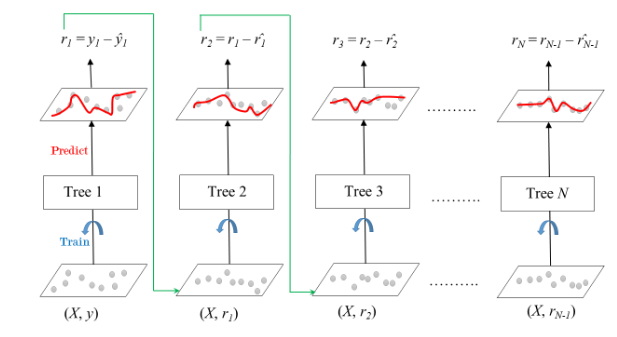
\includegraphics[width=0.75\linewidth]{images/gradientboosting.png}
    \caption{Illustration de l'algorithme de boost de gradient (\cite{geeksforgeeks2023gradient})}
    \label{fig:fig6}
\end{figure}

\subsection{Implémentation}
\label{chap4.sec4.sub2}
Le plus gros inconvénient des modèles non paramètriques en général est que le temps nécéssaire pour leur entraînement augmente avec la taille de l'ensemble d'entraînement et les techniques de boosting sont particulièrement démonstratifs de cette faille. Donc on utilise souvent des versions un peu modifiées, voir tronquées, de l'algorithme ci-dessus quand on a à faire à de grands ensembles de données (\cite{odegua2020predicting}). Pour ce projet j'ai donc utilisé l'implémentation de scikit-learn basée sur les histogrammes qui est plus efficace grâce à deux particularités majeures:

\begin{itemize}
    \item \textbf{Discrétisation des valeurs continues}: Les prédicateurs continues sont discrétisées en un nombre fixe de groupes au moment de la construction des arbres de décisions. Vous rappelez vous de l'exemple avec l'âge au début de la section \ref{chap4.section2}? Là où les arbres de décisions classiques utiliseraient chaque valeurs de ces prédicateurs comme branche. Le fait de créer des catégories pour les valeurs continues (catégories qui seront les branches de cet attribut) réduit la précision des valeurs des attributs mais permet un calcul beaucoup plus rapide.
    \item \textbf{Créer des histogrammes}: Pour chaque prédicateur, un histogramme\footnote{Un histogramme est un graphique qui montre la fréquence des données numériques à l'aide de rectangles. La hauteur d'un rectangle (l'axe vertical) représente la fréquence de distribution d'une variable (le montant ou la fréquence d'apparition de cette variable).} est construit en comptant le nombre d'exemples dans chaque branche, d'où le nom \textbf{Histogram-based Gradient Boosting}. Ces histogrammes sont la représentation qui sera utiliser pour entraîner les arbres au lieu de l'ensemble complet, cela permet de reduire significantivement l'usage mémoire et encore une fois d'accélérer l'entraînement des arbres. 
\end{itemize}

Traditionnellement, le prédicateur le plus important (lors de l'entraînement des arbres) est choisi comme étant celui qui minimise la somme de la somme quadratique des erreurs résiduelles dans chaque branche. Cette somme est définie par la formule: \[RSS = \Sigma_{n=1}^M Q_n\] où \(Q_n\) est la somme quadradique des erreurs résiduelles dans la \(n\)ième branche définie par: \[Q_n = \Sigma_i r_i^2\] où \(r_i\) est l'erreur résiduelle du \(i\)ème exemple de la branche. En pratique, pour les problèmes de classifications les erreurs résiduelles sont souvent remplacées par les gradients d'une \textbf{fonction de coût} et le but est de minimiser cette dernière, on détaillera cette approche dans la prochaine section.

Tout comme l'implémentation de la forêt aléatoire mon implémentation du boost de gradient possède 200 arbres, le taux d'apprentissage est fixé à 0,1 et le nombre maximal de groupes lors de la discrétisation des valeurs continues est fixé à 255; notez que cette limite est aussi applicable aux prédicateurs de nature catégorique possédant plus de 255 valeurs uniques(\cite{diarra2024gradient}).
\section{La régression linéaire}
\label{chap4.section5}
La régression linéaire est l’un des modèles paramétriques les plus anciens, peut-être même le modèle fondamental de cette philosophie. Elle a été introduite au début du XIXe siècle par le mathématicien et statisticien Francis Galton, qui l'a utilisée pour étudier la relation entre la taille des parents et celle de leur progéniture. Depuis lors, la régression linéaire a été largement étudiée et appliquée dans divers domaines, notamment l’économie et, bien sûr, l’apprentissage automatique.

Le but de la régression linéaire est de créer une approximation de la relation linéaire entre chaque variable indépendante et la variable dépendante, celà sous-entend donc que pour que la régression linéaire soit efficace les prédicateurs doivent décrire une certaine forme de linéarité avec la variable dépendante, c'est-à-dire une corrélation non nulle entre les variables d'entrées et la sortie. Lorsqu’il n’y a qu’une seule variable indépendante, on qualifie la tâche de: \textbf{\textit{Régression linéaire simple ou univariée}}. Et régression linéaire multi-variée s'il y a plus d'une variable d'entrée. Formellement, le problème de la régression linéaire est donc le suivant:

Étant donné un ensemble de données décrivant une corrélation linéaire entre des prédicateurs \(x_i\) et une variable de sortie (target) \(y\); trouver les valeurs des paramètres \(w_i\) et \(b\) pour lesquels l'équation linéaire \(y_j = b + \Sigma_i w_i \cdot x_{j,i}\) est vraie ou sensiblement vraie pour chaque exemple \(x_j\) dans l'ensemble d'entrainement. Les \(w_i\) sont appélés les \textbf{poids} et \(b\) le \textbf{bias} du modèle. Pour trouver ces valeurs, on cherche à minimiser une \textbf{fonction de coût}.

\subsection{Fonction de coût}
\label{chap4.sec5.sub1}
Une fonction de coût est un moyen de mésurer et de pondérer l'erreur d'un modèle, on l'appelle aussi fonction de perte. Une fonction de perte \(L(y, \hat{y})\) est définie comme l'utilité perdue en prédisant \(h(x)= \hat{y}\) lorsque la bonne réponse est \(f(x) = y\). Une fonction de perte est différente d’un taux d’erreur, dans le sens où une fonction de perte ne s’intéresse pas seulement à l’erreur du modèle en prédisant \(\hat{y}\) au lieu de \(y\). Toute fonction qui capture la perte réelle résultant d'une mauvaise prédiction du modèle peut être une fonction de perte.

Prenons l'exemple de notre thème même, le risque encouru par l'institution prêteuse en accordant un prêt à une personne qui s'avère être un prêt défaillant est beaucoup plus grand que celui qu'elle encourt en refusant un prêt à quelqu'un qui aurait potentiellement pu le rembourser, raison pour laquelle certaines institutions durcissent leur critères sur les prêts et refusent beaucoup de demandes. Et pareil au niveau du client les risque ne sont pas les mêmes, donc un modèle qui prédit beaucoup trop souvent des défauts de paiement comme bon prêt causera plus de tort dans le monde réel qu'un autre modèle qui a le bias inverse. On peut faire une fonction de perte qui capture cette subtilité, c'est là la différence entre une fonction de coût et le taux d'erreur, par exemple on peut définir une fonction de coût de manière à ce que \(L(y=remboursera, \hat{y}=!remboursera)=1\) and \(L(y=!remboursera, \hat{y}=remboursera)=10\).

La fonction de coût est la mésure de performance de l'apprentissage supervisé car dans beaucoup d'algorithmes c'est elle que nous cherchons à minimiser. Pour expliquer les différents concepts impliqués dans l'entraînement de tels modèles dans le reste de ce document, nous allons nous baser sur une des formes les plus simples de fonction de coût, la fonction de perte \(L2\) ou perte quadratique qui est définie comme: \[L2(y, \hat{y}) = (y - \hat{y})^2\] Lors d'un entraînement nous cherchons à minimiser la somme totale des pertes sur l'ensemble des données d'entraînement soit: \[SumL2 = \Sigma_j (y_j - \hat{y}_j)^2\]

Dans le context de la régression linéaire, on le rappelle \(\hat{y}_j = b + \Sigma_i w_i \cdot x_{j,i}\), ce qui donne comme perte: \[SumL2 = \Sigma_j (y_j - (b + \Sigma_i w_i \cdot x_{j,i}))^2\]

Cette somme étant une équation avec \(i+1\) inconnues, pour chaque poids \(w_i\) et un bias \(b\), elle atteint sa valeur minimale quand les dérivées partielles de la somme par rapport à chacune des inconnues sont égales à 0. C'est-à-dire lorsque: \[\frac{\partial}{\partial w_i} \Sigma_j (y_j - (b + \Sigma_i w_i \cdot x_{j,i}))^2 = 0\] pour chaque \(w_i\) de l'ensemble des poids et \[\frac{\partial}{\partial b} \Sigma_j (y_j - (b + \Sigma_i w_i \cdot x_{j,i}))^2 = 0\]

Ces équations ont une seule solution unique (si elle existe), souvent celà implique que les valeurs idéales des poids et du bias sont des nombres réels avec plus de 50 décimales, leur calcul prend donc énormement de temps et on est souvent obligés de les tronquer de toute façon. Donc au lieu de chercher directement les solutions de ces équations on cherche à les approximer grâce à un algorithme qu'on appelle la \textbf{descente de gradient} qui est devenu la norme avec les modèles paramétriques. L'idée est que, par exemple, si les vraies valeurs de \(w_1\) et \(b\) pour que leurs dérivées partielles respectives soient exactement égales à zéro sont: $w_1 = 1,702145614785401$ et $b = -0,8745123177559741$. Eh bien, nous serions assez satisfaits d'un algorithme qui convergerait vers $w_1 = 1,701$ et $b = -0,874$.

\subsection{La Descente de gradient}
\label{chap4.sec5.sub2}
Avec la descente de gradient, les valeurs des paramètres sont initialisées « aléatoirement » avec de petites valeurs, généralement issues d'une distribution gaussienne ou tout simplement mises à zéro au début de l'algorithme et nous visons à converger par itération vers une approximation des valeurs optimales des poids et du bias qui minimise la fonction de coût. L'algorithme est le suivant:

Pour un certain nombre d'époques\footnote{Une époque d'entraînement réfère à une application de l'algorithme de descente de gradient sur l'ensemble d'entraînement entier.} d'entraînement ou tant que l'algorithme n'a pas encore convergé (ce qui signifie qu'il y a encore des changements importants dans les valeurs des paramètres), on calculera les « gradients », c'est-à-dire les dérivées partielle de la fonction de perte pour chaque paramètres et chaque exemple d'entraînement \(x_j\) et on mettra à jour les valeurs de chaque \(w_i\) et de \(b\) suivant la direction de leurs gradients. Formellement ça donne l'algorithme suivant:

Pour m de 1 à \(M\) nombre d'époques
\begin{enumerate}
    \item \textbf{Calculer les gradients}: Calculer les gradients de la fonction de perte par rapport à chaque paramètres.
    
    \begin{itemize}
        \item Pour un exemple d'entraînment \(x_j\) et un certain \(w_i\), poids du \(i\)ème attribut de \(x_j\) on a donc: \[\frac{\partial}{\partial w_i} L2 = \frac{\partial}{\partial w_i} (y_j - (b + w_i \cdot x_{j,i}))^2 = 2(y_j - (b + w_i \cdot x_{j,i})) \cdot \frac{\partial}{\partial w_i} (y_j - (b + w_i \cdot x_{j,i}))\] \[= -2(y_j - (b + w_i \cdot x_{j,i})) \cdot x_{j,i}\]
        \item Pour le bias on a: \[\frac{\partial}{\partial b} L2 = \frac{\partial}{\partial b} (y_j - (b + w_i \cdot x_{j,i}))^2 = 2(y_j - (b + w_i \cdot x_{j,i})) \cdot \frac{\partial}{\partial b} (y_j - (b + w_i \cdot x_{j,i}))\] \[= -2(y_j - (b + w_i \cdot x_{j,i}))\]
    \end{itemize}
    
    Pour trouver les expressions ci-dessus il est juste nécéssaire de connaître les bases de la différentiation telles que: \(\frac{\partial}{\partial w} wx = x\) et \(\frac{\partial}{\partial w} w = 1\)
    
    \item \textbf{Mettre à jour les valeurs des paramètres}: Ensuite l'algorithme mettra à jour les valeurs des paramètres en utilisant la règle suivante:
    
    \begin{itemize}
        \item Pour chaque \(w_i\): \[w_i \leftarrow w_i - \eta \cdot \frac{\partial}{\partial w_i} L2\]
        \item Pour le bias: \[b \leftarrow b - \eta \cdot \frac{\partial}{\partial b} L2\] où \(\eta\) est le taux d'apprentissage, même principe que celui de la section \ref{chap4.sec4.sub1}
    \end{itemize}
    
\end{enumerate}

Une forme plus complète de l'algorithme est obtenu en sommant les mises à jours des poids pour chaque exemple d'entraînement \(x_j\) par rapport à la somme des pertes. Ce qui donne, pour \(j\) de 1 à \(N\) nombre d'exemples:

\begin{itemize}
    \item Pour chaque \(w_i\): \[w_i \leftarrow w_i - \eta \cdot \Sigma_j \frac{\partial}{\partial w_i} SumL2 = w_i + 2\eta \cdot \Sigma_j^N (y_j - (b + w_i \cdot x_{j,i})) \cdot x_{j,i}\]
    \item Pour \(b\): \[b \leftarrow b - \eta \cdot \Sigma_j \frac{\partial}{\partial b} SumL2 = b + 2\eta \cdot \Sigma_j^N (y_j - (b + w_i \cdot x_{j,i}))\]
\end{itemize}

En pratique, au lieu de répeter ces opérations pour chaque prédicateurs (donc pour chaque \(w_i\), ce qui va s'avérer très lent, on va plutôt vectorialiser toutes les équations précédentes depuis l'équation de prédiction du modèle. Ce qui va donner:

\begin{itemize}
    \item L'équation du modèles devient: \[\hat{Y} = b + W \cdot X\] où $W$ est la matrice des poids où \(w_{j,i}\) est le poids associé au $i$ème attribut du $j$ème exemple d'entraînement, \(X\) est la matrice de tous les exemples d'entraînement avec tous les prédicateurs, cette matrice est de la même forme que $W$, le bias reste une valeur unique pour tout l'ensemble et $\hat{Y}$ est le vecteur des prédictions sur l'ensemble entier, de manière similaire \(Y\) est le vecteur des vraies étiquettes.
    \item La formule de mise à jour des poids par la descente de gradient devient: \[W \leftarrow W - \eta \cdot \frac{\partial}{\partial W} SumL2 = W + 2\eta \cdot (Y - (b + W \cdot X)) \cdot X\] où \(W\) sera une matrice dont on pourra prendre la moyenne ou la somme par colonne comme nouvelle valeur des \(w_i\)
    \item La formule de mise à jour du bias par la descente de gradient devient: \[b \leftarrow b - \eta \cdot \frac{\partial}{\partial b} SumL2 = b + 2\eta \cdot (Y - (b + W \cdot X))\] où $b$ sera une matrice de bias dont on pourra ensuite prendre la moyenne ou la somme comme valeur unique pour $b$. Notez aussi que la plupart du temps on simplifie \(2\eta\) à \(\eta\) tout simplement car le taux d'apprentissage est généralement un nombre très petit dont la multiplication par 2 reste semblable à ce dernier.
\end{itemize}

En répétant donc le processus ci-dessus pour \(M\) iteration sur l'ensemble de données entier, \(M\) époque, l'algorithme de descente de gradient va converger vers les valeurs de chaque paramètres pour lesquelles la somme des pertes est minimiser. Il est plus facile de raisonner avec les formes simples de ces équations qu'avec leur formes matricielles donc pour les prochaines démonstration où on aura besoin de revenir à ces équations j'utiliserai les formes simples. La figure \ref{fig:fig7} montre une illustration d'un modèle de régression linéaire univariée entraîner pour prédire le prix d'une maison avec une seule variable indépendante qui est sa superficie. On peut voir que le modèle, alors définie par juste un poids et un bias, décrit une droite qui correspond presque parfaitement aux données d'entraînement et qui peut être utilisé pour prédire une estimation du prix d'une nouvelle maison. L'idée pour les modèles multi-variée aussi est de trouver les valeurs des paramètres de l'hyperplan\footnote{En géométrie, un hyperplan est une généralisation d'un plan bidimensionnel dans un espace tridimensionnel à des espaces mathématiques de dimension arbitraire. Comme un plan dans l'espace, un hyperplan est une hypersurface plate, un sous-espace dont la dimension est inférieure d'une unité à celle de l'espace ambiant. Dans un espace bidimensionnel, c'est une ligne; dans un espace tridimensionnel, c'est un plan, et ainsi de suite.} qui décrit le même comportement pour un espace multi-dimensionnel.

\begin{figure}
    \centering
    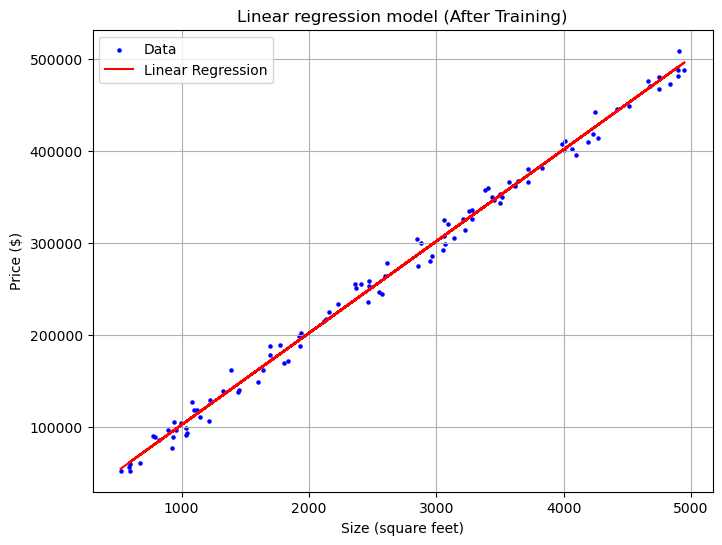
\includegraphics[width=0.75\linewidth]{images/linreg.png}
    \caption{Un modèle de régression linéaire simple décrit une droite qui suit la relation linéaire de l'ensemble de données}
    \label{fig:fig7}
\end{figure}

Tout comme pour les arbres de décisions je n'ai pas implémenté de modèle de régression linéaire pour ce projet. Comme son nom l'indique la régression linéaire est un algorithme de régression et la tâche de prédire les défauts de paiement est une tâche de classification, cependant expliquer la régression linéaire en profondeur comme ici me permettra d'être plus concis dans les explications des trois dernier modèles que j'ai testé.
\section{La régression logistique}
\label{chap4.section6}
De par le fait qu'ils sont caractérisés par une ensemble fixe de paramètres (généralement égal au nombre de prédicateurs + 1 bias), les modèles de régression linéaire sont obligés de construire une hypothèse forte sur la fonction inconnue qui a génère les données. Parce que contrairement aux modèles non paramètriques comme les arbres de décisions, ils n'ont pas la capacité de changer de forme ou de grandir pour s'adapter parfaitement à l'ensemble d'entraînement, donc ils doivent faire des compromis pour trouver les meilleurs approximations des valeurs de poids et du bias qui minimise les pertes pour tous les exemples d'entraînement.

Cette particularité qui est censé être une contrainte de base s'avère finalement être la meilleure solution face au sur-ajustement. En effet ces modèles sont beaucoup moins sensible à ce problème, tout en faisant des prédictions correctes la plupart du temps. On veut pouvoir mettre ce type de modèle au service des problèmes de classification également, il y'a donc deux possibilités majeures qui s'offre à nous: le \textbf{seuillage} ou la conversion de prédictions réelle continues en \textbf{probabilité}.

Avec la regression logistique on choisit la deuxième option afin de pouvoir faire de cette conversion une partie intégrante du modèle. Plus exactement, la régression logistique est une modification de la régression linéaire parfaitement pensée pour les problèmes de classification binaire (comme prédire les défaut de paiement). L'idée est de prendre un modèle de régression linéaire et de l'équiper d'une fonction qui puisse transformer la sortie \(\hat{y}_j = b + \Sigma_i w_i \cdot x_{j,i}\) en la probabilité que l'exemple \(x_j\) appartienne à la classe positif. Cette fonction est connue sous le nom de fonction \textbf{sigmoid} et est définie par: \[Sigmoid(z) = \frac{1}{1 + e^{-z}}\] C'est bien la fonction de la fin de l'algorithme \ref{chap4.sec4.sub1}. Vous pouvez remarquez que quelque soit la valeur de \(z\) les valeurs de cette fonction sont dans l'intervalle \(]0, 1[\).

En grosso modo, l'idée est de modifier légèrement un modèle de régression linéaire de manière à ce que les prédictions du modèle soit désormais sous la forme \(Sigmoid(z)\) où \(z = \hat{y}_j = b + \Sigma_i w_i \cdot x_{j,i}\) représentant la probabilité que l'exemple \(x_j\) appartienne à la classe positif (représentée par 1) qui dans notre cas signifie que le client fera défaut sur son prêt. La figure \ref{fig:fig8} montre l'effet de la fonction sigmoid sur les prédictions du modèle de régression et comment ces probabilités sont typiquement interprêtées.

\begin{figure}
    \centering
    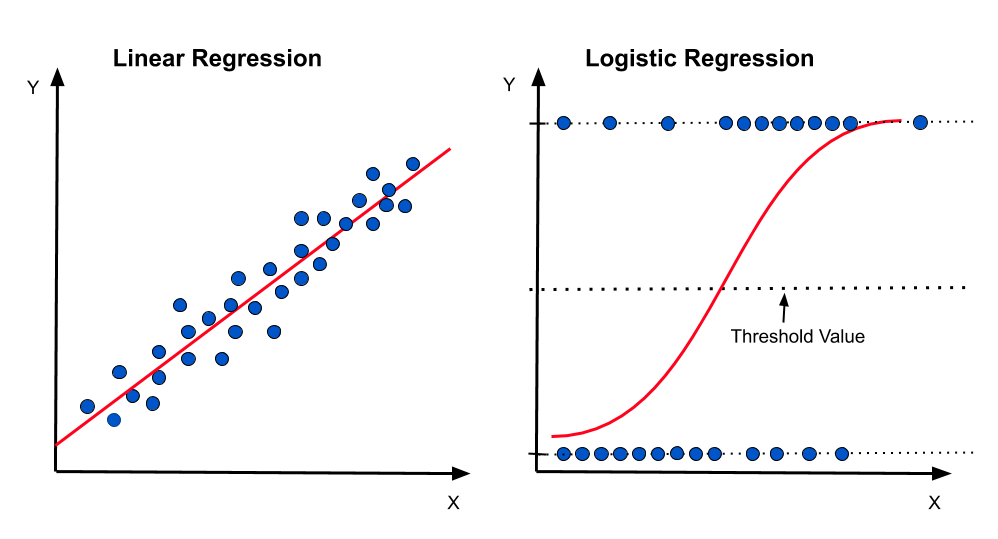
\includegraphics[width=0.75\linewidth]{images/logitReg.png}
    \caption{Visualisation d'un modèle de régression logistique simple}
    \label{fig:fig8}
\end{figure}

\subsection{Algorithme (Descente de gradient)}
\label{chap4.sec6.sub1}
Le concept et l'algorithme de descente de gradient utilisé pour entraîner le modèle reste fondamentalement le même. Il y'a juste une petite nouvouté, puisque maintenant la prédiction du modèle n'est plus donnée directement par \(\hat{y}_j = b + \Sigma_i w_i \cdot x_{j,i}\) mais plutôt par \(Sigmoid(\hat{y}_j)\) on va avoir besoin d'une étape supplémentaire pour trouver le gradient de la fonction de perte par rapport aux différents poids et au bias parce que la fonction de coût \(L2\) qu'on va encore utilisée pour l'illustration elle est toujours en fonction de \(\hat{y}_j\) comme toute autre fonction de coût en soit. Ce qui nous amène au calcul suivant:

\begin{itemize}
    \item Pour un exemple d’entraînment \(x_j\) et un certain \(w_i\), poids du \(i\)ème attribut de \(x_j\) on a donc: \[\frac{\partial}{\partial w_i} L2 = \frac{\partial L2}{\partial Sigmoid(\hat{y}_j)} \cdot \frac{\partial Sigmoid(\hat{y}_j)}{\partial \hat{y}_j} \cdot \frac{\partial \hat{y}_j}{\partial w_i}\]
    \item Pour le bias on a: \[\frac{\partial}{\partial b} L2 = \frac{\partial L2}{\partial Sigmoid(\hat{y}_j)} \cdot \frac{\partial Sigmoid(\hat{y}_j)}{\partial \hat{y}_j} \cdot \frac{\partial \hat{y}_j}{\partial b}\]
\end{itemize}

Avec les démonstrations de la section \ref{chap4.sec5.sub2} on sait que:  \[\frac{\partial L2}{\partial Sigmoid(\hat{y}_j)} = \frac{\partial}{\partial Sigmoid(\hat{y}_j)} (y_j - Sigmoid(\hat{y}_j))^2 = -2(y_j - Sigmoid(\hat{y}_j))\]
\[\frac{\partial \hat{y}_j}{\partial w_i} = \frac{\partial}{\partial w_i} (b + w_i \cdot x_{j,i}) = x_{j,i}\]
\[\frac{\partial \hat{y}_j}{\partial b} = \frac{\partial}{\partial b} (b + w_i \cdot x_{j,i}) = 1\]

Il ne reste donc plus qu'à dériver la fonction sigmoid par rapport à \(\hat{y}_j\), on obtient donc: \[(Sigmoid(\hat{y}_j))' = (\frac{1}{1 + e^{-\hat{y}_j}})' = \frac{-(-e^{-\hat{y}_j})}{(1 + e^{-\hat{y}_j})^2} = \frac{e^{-\hat{y}_j}}{(1 + e^{-\hat{y}_j})^2}\]

Au final on obtient:

\begin{itemize}
    \item Pour un exemple d’entraînment \(x_j\) et un certain \(w_i\), poids du \(i\)ème attribut de \(x_j\): \[\frac{\partial}{\partial w_i} L2 = -2(y_j - Sigmoid(\hat{y}_j)) \cdot \frac{e^{-\hat{y}_j}}{(1 + e^{-\hat{y}_j})^2} \cdot x_{j,i}\]
    \item Pour le bias: \[\frac{\partial}{\partial b} L2 = -2(y_j - Sigmoid(\hat{y}_j)) \cdot \frac{e^{-\hat{y}_j}}{(1 + e^{-\hat{y}_j})^2}\]
\end{itemize}

L'algorithme de descente de gradient reste exactement le même et les mêmes concepts s'applique. Ce qui est très intéressant avec les nouveaux modèles et démonstrations qu'on voit depuis le section \ref{chap4.section5} c'est qu'on peut remarquer que ces concepts et algorithmes peuvent se généraliser à d'autres fonctions et problèmes. Donc il est techniquement possible de remplacer la fonction \(L2\) et la fonction \(Sigmoid\) avec n'importe quelle autre fonction différentiable. Cela a permit le développement de d'autres algorithmes comme les réseaux de neuronnes artificiels.

\subsection{Implémentation}
\label{chap4.sec6.sub2}
Mon implémentation de la régression logistique est assez « peu conventionnelle » on va dire, puisque je l'ai implémenté avec keras qui est un framework (une structure) pour l'apprentissage profond normalement (\cite{chollet2015keras}). Cela a donné un modèle avec des particularités qu'on associe typiquement aux réseaux de neuronnes, par exemple la descente de gradient est éffectuée par l'algorithme du \textbf{Moment adaptatif (AdaM)} qui est une version légèrement modifiée de l'algorithme de descente de gradient ordianaire décrit dans la section \ref{chap4.sec5.sub2}; de plus la mise à jour des paramètres se fait par lot, c'est-à-dire que les gradients sont accumulés et la descente se fait pour un lot à la fois, qui est une matrice de \(M\) exemples d'entraînement sur \(N\) au total au lieu de le faire pour chaque exemple individuellement ou pour une grande matrice de tout l'ensemble comme je l'avais précédemment évoqué. Ceci étant dit le fonctionnement du modèle est conceptuellement identique à celui d'un modèle de regression logistique et peut donc être considéré comme tel.

La raison pour laquelle j'ai décidé d'implémenter la régression logistique comme ceci est de faciliter la transition vers les réseaux de neuronnes dans ce document et pour ceux qui liront les codes.

Mon implémentation utilise aussi une fonction de coût différente de \(L2\) qui est pensée particulièrement pour les problèmes de classification et classification binaire notamment. C'est la fonction de \textbf{cross-entropie binaire} ou log-loss définie par: \[LogLoss = - [y_j \cdot log(p_j) + (1 − y_j)\cdot log(1−p_j)]\] où \(p_j = Sigmoid(\hat{y}_j)\) et donc la forme complète est la somme normalisée des pertes: \[LogLoss = - \frac{1}{N} \Sigma_j^N [y_j \cdot log(p_j) + (1 − y_j)\cdot log(1−p_j)]\] où \(N\) est le nombre d'exemple. De par son expression cette fonction de perte atteint sa valeur maximal quand \(y_j\) est trop différent de \(p_j\), une manière de pénaliser plus lourdement le modèle quand il a gravement tort et donc d'avoir des gradients plus grands pour rémedier à ça.

Le modèle a donc été entraîner sur ces bases là pour sept (07) époques sur des lots de 64 exemples et avec un taux d'apprentissage de 0,001 (\cite{diarra2024notebooks}).
\section{Les réseaux de neurones artificiels}
\label{chap4.section7}
Revenons au modèle de régression logistique de la section \ref{chap4.section6}, maintenant au lieu de le voir comme un modèle à part entière je vous suggère de penser à ce modèle comme une simple unité de calcul, une petite partie d'un modèle beaucoup plus grand. C'est assez peu commun d'expliquer les résaux neuronaux de cette manière mais c'est bien là les fondements de cet algorithme.

\begin{figure}
    \centering
    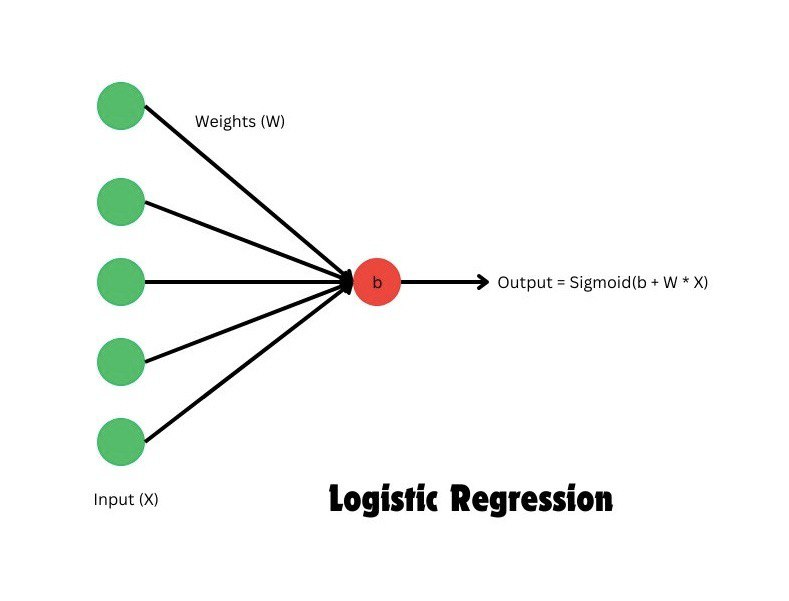
\includegraphics[width=0.75\linewidth]{images/logitReg2.png}
    \caption{Un modèle de régression logistique vu comme un neuronne}
    \label{fig:fig9}
\end{figure}

Les réseaux de neuronnes artificiels sont un type de modèle paramétriques qui marche grâce à la superposition de plusieurs couches de petites unités de calcul qui sont traversées une à une par les différents attributs \(x_{j,i}\) d'un exemple de donnée \(x_j\). Les sorties d'une couche devenant les entrées de la suivante jusqu'à une couche de sortie représentant la prédiction du modèle pour l'exemple \(x_j\) (cette couche peut aussi contenir plusieurs unités de calculs). Ce sont les fondements de toute une famille d'algorithmes basés sur ce concept et d'un sous domaine de l'apprentissage automatique appélé: \textbf{Apprentissage profond}\footnote{L'apprentissage profond est un sous domaine de l'apprentissage qui utilise des réseaux neuronaux artificiels et d'autres algorithmes compexes pour simuler le pouvoir de décision complexe du cerveau humain. Ce genre de modèle alimente la majeure partie de l’intelligence artificielle aujourd’hui.}.

Les unités de calcul vont être appélées « neuronnes » et le type de modèle que je décris dans le paragraphe précédent est le type de modèle d'apprentissage profond le plus simple appélé: réseau neuronal à action directe ou \textbf{feedforward neural network}. Comme je l'ai dit dans la section \ref{chap4.sec6.sub2}, l'implémentation que j'ai fait de la régression logistique était faite ainsi dans le but de faciliter l'analogie et la transition aux réseaux de neuronnes. En effet si l'on considère un modèle de régression logistique comme un seul neuronne unique comme l'illustre la figure \ref{fig:fig9}, il dévient beaucoup plus simple de raisonner avec les réseaux neuronaux à action directe,  vous pouvez les voir comme des modèles qui superpose plusieurs modèles de régression logistique (neuronnes) par couche. La figure \ref{fig:fig10} montre un réseau neuronal directe avec 2 couches intermédiaires ou couches cachées \textit{(hidden layers)} et un seul neuronne de sortie pensé pour la classification binaire.

\begin{figure}
    \centering
    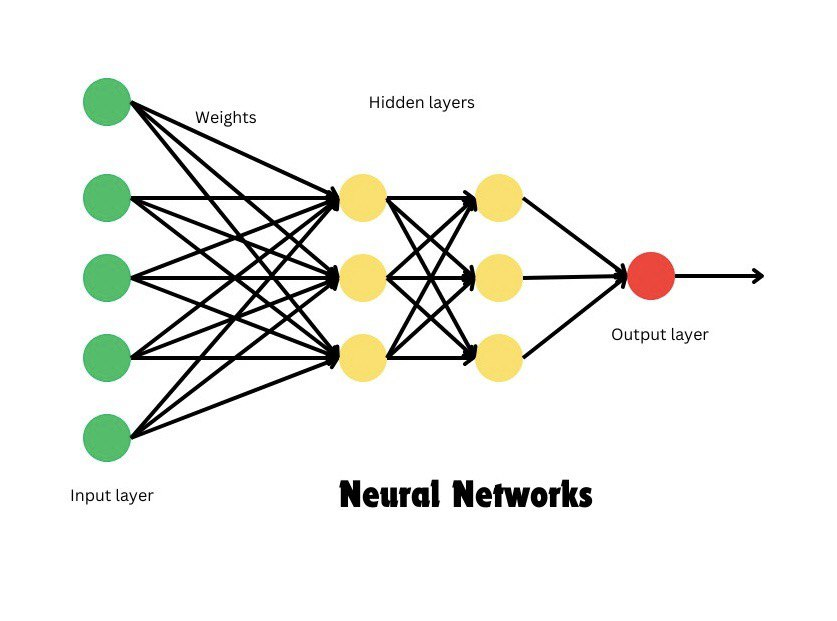
\includegraphics[width=0.75\linewidth]{images/neuralnet.png}
    \caption{Un réseau neuronal à action directe vu comme un ensemble de modèle de régression logistique}
    \label{fig:fig10}
\end{figure}

Ajoutez à celà le fait qu'on a la possibilité de remplacer la fonction sigmoid par toute autre fonction pour chaque neuronne en théorie (même si en pratique et par covention les neuronnes de la même couche utilisent la même fonction) et on a toutes les bases de l'apprentissage profond. Pour un neuronne la fonction qui permet de passer de \(\hat{y}_j = b + \Sigma_i w_i \cdot x_{j,i}\) à l'entrée du prochain neuronne est ce qu'on appelle une \textbf{fonction d'activation}. Pour simplifier les démonstrations dans ce document on va supposer que toutes les fonctions d'activations sont la fonction sigmoid.

\subsection{La rétro-propagation}
\label{chap4.sec7.sub1}
La rétro-propagation est une variante de l'algorithme de descente de gradient qui vise à adapter cette dernière à l'entraînement de réseaux de neuronnes multi-couches (\cite{nielse2018nneural}). L'algorithme est presque identique à la descente de gradient, juste qu'il apporte un support pour calculer les gradients des poids et des bias qui n'appartienne pas au neuronne de la couche de sortie en propageant l'erreur de la dernière couche aux précédentes grâce à ses gradients, d'où le non \textbf{rétro-propagation}. L'algorithme de rétro-propagation appliqué au poids et au bias du neuronne de sortie qui prédit la probabilité qu'un exemple \(x_j\) appartienne à la classe positive revient à la descente de gradient sur un modèle de régression logistique.

Avez vous pris soins de remarquer cette expression dans la section \ref{chap4.sec6.sub2}? \[\frac{\partial}{\partial w_i} L2 = \frac{\partial L2}{\partial Sigmoid(\hat{y}_j)} \cdot \frac{\partial Sigmoid(\hat{y}_j)}{\partial \hat{y}_j} \cdot \frac{\partial \hat{y}_j}{\partial w_i}\] Cette décomposition est connu sous le nom de: \textbf{règle de la chaîne des gradients} et elle est le fondement de l'algorithme de rétro-propagation car en interpolant ainsi des termes qui font le lien entre la fonction de perte et un poids ou un bias donné on peut trouver les expressions des gradients de fonction de perte par rapport à n'importe quel poids ou bias du réseau neuronal. L'algortihme de rétro-propagation appliqué aux couches cachées du réseau revient donc simplement à suivre la chaîne. Ce qui est en revanche très fastidieux puisque la chaîne s'aggrandit au fur et à mésure qu'on remonte dans le réseau. 

Tout cela paraît assez complexe pour quelqu'un qui n'est pas particulièrement bon en math et croyez moi j'ai souffert pour en arriver à ce petit niveau de compréhension. En résumé, la seule réelle différence entre l'algorithme de rétro-propagation et la descente de gradient est la taille de la chaîne des gradients. Les autres étapes une fois qu'on a les gradients de la fonction de perte par rapport à tous les poids et tous les bias restent identiques à la descente de gradient vu dans la section \ref{chap4.sec5.sub2}.

\subsection{Implémentation}
\label{chap4.sec7.sub2}
Comme dit précédemment, j'ai fait une implémentation avec keras d'un réseau de neuronnes à action directe. Après plusieurs tests, l'architecture qui conciliait les performances et le temps d'entraînement du modèle est composée d'une seule couche cachée de 100 neuronnes et d'une couche de sortie avec un seul neuronne. Les neuronnes de la couche cachée ont comme fonction d'activation la fonction d'unité linéaire rectifiée (\textbf{relu}) définie comme: \[relu(z) = max(0, z)\] En plus d'introduire une forme de non linéarité dans le fonctionnement du modèle, la fonction d'unité linéaire rectifiée et ses variantes sont généralement préférées pour les couches cachées en raison de la simplicité de leurs gradients ce qui permet d'accélerer considérablement la descente de gradient.

Pour l'unique neuronne de sortie, cela va de soit, la fonction sigmoid s'impose pour que les prédictions finales du modèle puisse être interprêtées comme la probabilité d'un exemple donnée de faire défaut sur son prêt. Et puisque le problème reste une classification binaire la fonction de coût reste la même que pour la régression logistique à savoir \textbf{log-loss}. Le meilleur modèle a été entraîner pour 10 époques d'entraînement sur des lots de 64 exemples par descente de gradient et avec un taux d'apprentissage de 0,001 encore une fois (\cite{diarra2024notebooks}).
\section{Les machines à vecteur de support}
\label{chap4.section8}
Les machines à vecteur de support (\textbf{SVMs}) sont une famille d'algorithmes de classification dont l'objectif principal est de trouver une hyperplan qui sépare les exemples des différentes classes de manière optimale. Pour cela les SVMs cherchent à maximiser la marge, c'est-à-dire la distance entre l'hyperplan et les points de données (exemples) les plus proches de chaque classe. Ces points les plus proches sont appelés \textbf{vecteurs de support}. L'algorithme général peut être décrit comme suit:

\begin{enumerate}
    \item Quand l'ensemble de données est directement linéairement séparable, les SVMs cherchent à trouver les bonnes valeurs des paramètres \(w_i\) et \(b\) de l'hyperplan \[b + \Sigma_i w_i \cdot x_i = 0\] qui maximise la marge. Les \(x_i\) sont les attributs ou prédicateurs de l'ensemble de données. Ceci est formulé comme un problème d'optimisation où la fonction à minimiser est: \[\frac{1}{2} \Sigma_i ||w_i||^2\] sous contraintes \[y_j(b + \Sigma_i w_i \cdot x_{j,i}) \geq 1\] pour tout exemple \(x_j\). 
    \item Quand l'ensemble de données n'est pas directement linéairement séparable, les SVMs utilisent des fonctions pour transformer les données dans un espace dimensionnel plus grand où elles peuvent être séparées linéairement.
    \item Pour les ensembles de données non linéairement séparables, les SVMs introduisent des variables de relâchement \(\zeta_i\) pour permettre certaines violations de la marge. Le problème de minimisation dévient donc: \[min(\frac{1}{2} \Sigma_i ||w_i||^2 + \epsilon \cdot \zeta_i)\] où \(\epsilon\) est un paramètre qui contrôle le compromis entre maximiser la marge et minimiser les erreurs de classification. Encore une fois sous les contraintes: \[y_j(b + \Sigma_i w_i \cdot x_{j,i}) \geq 1 - \zeta_i; et \zeta_i \geq 0\]
\end{enumerate}

La figure \ref{fig:fig11} montre une illustration de l'algorithme général appliqué à des données linéairement séparable pour une classification binaire. En pratique une approximation des valeurs des \(w_i\) et \(b\) grâce à la descente de gradient est toujours possible et toujours préférable avec les grands ensembles de données.

\begin{figure}
    \centering
    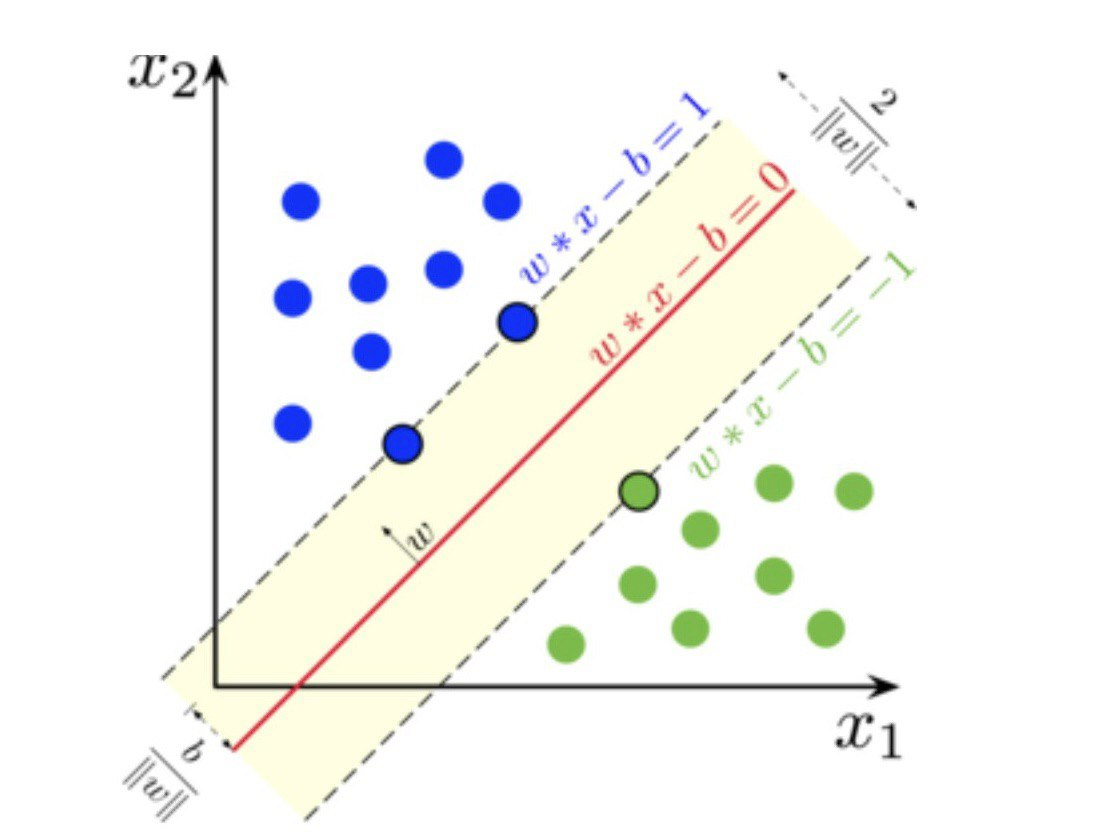
\includegraphics[width=0.75\linewidth]{images/SVM_margin.jpg}
    \caption{Machines à vecteur de support pour une classification binaire}
    \label{fig:fig11}
\end{figure}

\subsection{Les machines à vecteur de support pour la détection d'anomalie}
\label{chap4.sec8.sub1}
Un détail que je n'ai pas précisé avec les autres modèles est que l'ensemble de données que j'avais à disposition pour ce travail était très déséquilibré. Sur les 1.526.659 exemples il n'y avait que 47.994 qui avait faillit sur leur prêt, soit approximativement 3\% de l'ensemble de données. C'est une situation qui peut arriver dans certaines applications où les différentes classes sont naturellement déséquilibrés, la section \ref{chap4.section9} sera dédiée à expliquer ce problème et les solutions que j'ai mis en place pour essayer de minimiser l'impact sur les modèles de classification.

Cette section n'était pas censé faire partie du document initialement, tout vient de l'idée qu'avec un ensemble de données si déséquilibré, un modèle de detection d'anomalies\footnote{La détection d'anomalies est un domaine essentiel de l'analyse de données et de l'apprentissage automatique, qui consiste à identifier des observations ou des événements rares et atypiques dans un ensemble de données. Ces anomalies peuvent indiquer des erreurs, des fraudes, des pannes ou d'autres phénomènes inhabituels qui nécessitent une attention particulière.} pourrait s'averer meilleur pour distinguer les deux classes. Donc l'idée m'a été proposer d'implémenter un modèle de detection d'anomalies qui sera utiliser comme un modèle de classification dans le soucis de déterminer correctement les clients qui sont plus susceptibles de faire défaut sur leur prêt.

Dans un papier de 1999, Bernhard Scholkopf et al ont proposé un algorithme de machine à vecteur de support pour aborder le problème de détection d'anomalies en essayant d'estimer un
fonction \(f\) qui est positive sur un sous-ensemble \(S\) des données (considéré comme normal) et négative sur le complément (considéré comme anomalie). Leur méthode est un algorithme d'apprentissage non supervisé qui prend un ensemble de données \(X\) le projette dans un espace dimensionnel plus grand et cherche les paramètres de l'hyperplan qui englobe la majeur partie des données tout en maximisant la marge entre les points de données et l'origine de l'espace dimensionnel (\cite{scholkopf1999support}). Le resultat est un modèle qui, une fois entraîné, évalue si un nouveau point de donnée tombe dans cet hyperplan (normal) ou à l'extérieur (anomalie).

\subsection{Impémentation}
\label{chap4.sec8.sub2}
J'ai donc testé cet algorithme, en entraînant un modèle sur un sous-ensemble des clients qui avait remboursé leurs prêts (un peu à la dernière minute), ce qui a justifié l'ajout de cette section. L'implémentation est basé sur celle de scikit-learn de l'algorithme de Scholkopf et al. Par contre l'algorithme est très inefficace en termes de temps ce qui m'a obligé à entraîner seulement sur 100.000 exemples (\cite{diarra2024anomaly}).
\section{Gérer le déséquilibre des données}
\label{chap4.section9}
Comme je l'ai évoqué dans la section \ref{chap4.sec8.sub1}, le déséquilibre des données est un aspects pas si rare que cela avec les ensemble de données. Enfaîte certains ensembles de données le sont ne serait-ce que de par la nature de la tâche que l'on cherche à faire avec, par exemple la detection de tumeurs par images. Dans cette application de la vision par ordinateur, l'ensemble de données est typiquement constitué d'images d'échographies (entre autres) où chaque pixel est étiquetté comme cancereux ou non selon la zone de l'image qui est atteint d'une tumeur sur le corps du patient. Dans un dataset pareil, des millions de pixels vont être étiquetté comme "normal" là où à peine un millier portera l'étiquette inverse et heureusement d'ailleurs, on ne souhaite pas que les gens ait des cancers énormes.

On parle donc d'ensemble de données déséquilibré quand une étiquette en particulier est très largement en supériorité numérique par rapport à l'autre ou aux autres. Ce déséquilibre en lui même apporte des informations, que ce soit sur la manière dont les données ont été collectées, le lieu et même des informations sur la fonction qui génère les données.

Cependant ce déséquilibre pose un problème pour l'apprentissage des modèles, du fait de la rarété de la classe minoritaire, les algorithmes que nous avons vu de la section \ref{chap4.section2} à \ref{chap4.section7}, qui sont des algorithmes de classification vont vite même très vite converger vers le minimum de leur fonction de perte sans pour autant que le modèle résultant n'est appris quoi que ce soit des données. Les données fournies par Home Credit Group contenait des informations sur plus d'un million et demi de demandes de prêt parmi lesquelles juste 3\% ont échoué à rembourser le prêt accordé. D'un côté on est bien content pour eux parce que ça veut dire que Home Credit Group et leur clients gèrent très bien les crédits mais de l'autre ça complique la tâche de l'ingénieur en apprentissage automatique de dévélopper un modèle qui puisse réellement distinguer les bons des mauvais crédits.

Vous l'avez surêment déviné, le problème avec les ensembles de données déséquilibrés est que ils exploitent le plus gros hack\footnote{Un hack est une stratégie construite sur une faille d'un système afin de détourner ce dernier ce son fonctionnement normal ou de produire d'autres éffets qui n'avait pas été anticipés par le créateur du système. Le mot vient du verbe anglais \textbf{to hack} qui veut dire forcer un système.} des algorithmes d'apprentissage supervisé: \textbf{la fonction de perte}. En éffet pour qu'une fonction de perte d'un problème d'apprentissage supervisé puisse permettre d'extraire des connaissances des données dans un problème de classification, les différentes classes sont assumées d'avoir la même probabilité dans l'ensemble de données de sorte à ce que le pire qu'un modèle puisse avoir en termes de justesse de classification en prédisant toujours la même classe soit égale à cette probabilité.

Pour prendre l'exemple sur notre problème de classification binaire, la fonction log-loss est pensée de sorte à ce qu'un modèle qui prédit toujours la même classe (disons la classe 0 par exemple) est une perte totale extrêmement grande pour l'ensemble (en supposant que ce dernier est équilibré). Vous vous rappelez de l'expression de la fonction log-loss à la fin de le section \ref{chap4.sec6.sub2}?

Un modèle qui prédit toujours la classe 0, disant donc que le client remboursera son prêt, a une probabilité de prédiction de 1 (100\%) pour la classe 0 et de 0 (0\%) pour la classe 1. Ce qui donne une perte égale à 0 pour la classe 0 et \(\infty\) pour la classe 1. En théorie \(log(0)\) n'est pas définie et l'infini n'est pas un nombre, mais dans notre context ici on aura pas à ce préoccuper de ça car comme je l'ai dit \(p_j\) dans la formule de log-loss est la prediction du modèle qui est donnée uniquement comme la probabilité que le l'exemple \(x_j\) appartienne à la classe 1. Et cette probabilité est donné par la fonction sigmoid qui elle ne varie que dans l'intervalle ouvert ]0,1[ (signifiant que 0 et 1 sont exclus). Donc en pratique un modèle qui prédit tout le temps la classe 0 est un modèle qui donne toujours une très faible probabilité de la classe 1, pour simplifier ici va choisir \(p_j = 0,0001\). Donc pour un modèle de classification qui prédit tout le temps la classe 0 avec \(p_j = 0,0001\), en supposant un ensemble de données équilibré de \(N\) exemples, on a:

\begin{itemize}
    \item Pour tous les exemples de la classe 0:\[LogLoss = - [0 \cdot log(0,0001) + (1 − 0)\cdot log(1−0,0001)] = 0,0001 \approx 0\]
    \item Pour tous les exemples de la classe 1: :\[LogLoss = - [1 \cdot log(0,0001) + (1 − 1)\cdot log(1−0,0001)] = 9,21\]
    \item Pour l'ensemble: \[LogLoss = \frac{1}{N}(\frac{N}{2} \cdot 0 + \frac{N}{2} \cdot 9,21) = \frac{1}{N}(\frac{N}{2} \cdot 9,21) = \frac{9,21}{2} \approx 4,605\] Pour une fonction dont le minimun est autour de zéro on est bien loin, cela implique que ce modèle aura raison 50\% du temps en prédisant la même classe puisque l'ensemble est équilibré mais une perte totale de presque 5 et on le rappelle le but est de minimiser la fonction de perte ce qui conduira l'apprentissage.
\end{itemize}

En révanche le même modèle avec un ensemble déséquilibré sera dans un confort énorme qui ne permettra pas d'apprentissage. En supposant maintenant qu'on a un ensemble avec 97\% de classe 0 comme avec celui de Home Credit Group. La perte totale du modèle sera approximativement: \[LogLoss = \frac{1}{N}(\frac{9,7 N}{10} \cdot 0 + \frac{0,3 N}{10} \cdot 9,21) = \frac{1}{N}(\frac{0,3 N}{10} \cdot 9,21) = \frac{0,3 \times 9,21}{10} \approx 0,27\]

C'est la même fonction de coût, le même modèle en termes de compétences mais deux réalités très différentes. Dans le second cas le modèle sera dans une sorte de confort qu'il n'a pas dans le premier cas, car l'algorithme lui fera comprendre que les pertes sont déjà proches du minimum alors que le modèle n'a pas plus de pouvoir de prédiction que si l'on jouait la décision à pile ou face dans le fond. Le modèle comprend donc qu'en ne faisant aucun éffort dans ce nouvel environnement il a quand même raison 97\% du temps et les pertes sont minimisées.

Cette situation est la raison pour laquelle j'ai décidé d'implémenter l'algorithme décrit dans la section \ref{chap4.sec8.sub1} en tant que système de classification. Car si tous les algorithmes supervisés de classification sont sujets au problème décrit ci-haut avec les ensemble de données déséquilibrés (car ils ont tous dans le fond le même objectif). Un algorithme de détection d'anomalies non supervisé, de par sa nature même n'y est pas confronté et sera donc (en théorie) plus capable de reconnaître les exemples de la classe 1 (positifs). La section 5.2 fournit une évaluation comparative des différents modèles. Mais avant donc d'en arriver à détourner un algorithme de detection d'anomalies pour faire de la classification, j'ai essayé certains techniques pour tenter de minimiser l'impact du déséquilibre sur les modèles de classification.

\subsection{Sur et sous échantillonnage}
\label{chap4.sec9.sub1}
Le \textbf{sous-échantillonnage} est une technique conçue pour éssayer de gérer les ensembles de données déséquilibrés lors de l'entraînement de modèle de classification. Différentes implémentations existent mais l'idée de base est de supprimer certains exemples de la classe majoritaire jusqu'à atteindre une certaine forme d'équilibre. Ces exemples peuvent être supprimer soit aléatoirement (au risque de perdre des exemples intéressants) soit selon quelques critères comme par exemple supprimer les exemples de la classe majoritaire qui sont trop proches d'un ou plusieurs exemples de la classe minoritaire de par les valeurs de leur attributs.

Le \textbf{sur-échantillonnage} est la technique inverse, dans sa forme la plus simple elle consiste juste à répéter certains exemples de la classe minoritaire dans l'ensemble de données de manière aléatoire jusqu'à atteindre l'équilibre. D'autres variantes permettent de générer des exemples de la classe minoritaire en fonction de ceux qui sont déjà présents, dans cette catégorie le plus connu est sans doute \textbf{SMOTE} ou la technique de suréchantillonnage minoritaire synthétique de son nom complet en français. Avec SMOTE l'idée est de générer synthétiquement un exemple qu'on attribut à la classe minoritaire en faisant la différence entres les valeurs des prédicateurs d'un exemple de la classe minoritaire et un ou plusieurs de ses plus proches voisins dans l'espace des prédicateurs (en fonction du nombre d'exemple qu'on veut générer) et de multiplier toutes les valeurs obtenues par un nombre réelle choisit au hasard entre 0 et 1. Les valeurs obtenues à la fin seront les valeurs des prédicateurs d'un nouvel exemple qui sera attribuer à la classe minoritaire (\cite{chawla2002smote}).

Les deux familles de techniques permettent de passer d'un ensemble de données déséquilibré à un autre qu'on a donc forcé à être équilibré, mettant les algorithmes de classification dans leur zone de confort pour qu'ils puissent apprendre à distinguer les différentes classes. En revanche, pour un ensemble de données qui par nature est déséquilibré, c'est-à-dire que le déséquilibre des données ne vient pas de la méthode de collecte mais d'une réalité du terrain, l'utilisation des techniques de sur et sous ajustements présente le risque d'entraîner et de valider un modèle qui va au final drastiquement chuter en performances quand il sera de nouveau confronté à un ensemble de données déséquilibré. Particulièrement si les prédicateurs n'ont pas été assez travaillés ou qu'ils entretiennent des rélations complexes avec la variable dépendante, dans ce genre de cas équilibrer les données peut donc devenir l'arbre qui cache la forêt.

J'ai été confronté à ce problème en utilisant ces techniques, j'ai donc décidé de ne pas tenter d'équilibrer l'ensemble de données et d'essayer de construire des modèles de classification correctes et conforme à la réalité de l'ensemble déséquilibré. Pour cela j'ai adopté une autre technique mathématiquement beaucoup plus fiable.

\subsection{Pondérer les classes}
\label{chap4.sec9.sub2}
La technique que j'ai finalement utilisé pour essayer de minimiser l'impact du déséquilibre des données sur les modèles de classification attaque directement la source du problème à savoir la fonction de coût. L'idée est de fixer un poids sur les erreurs du modèles de sorte à ce que l'erreur de classifier un exemple de la classe 1 soit beaucoup plus grande que l'erreur inverse. Si vous vous rappelez bien j'avais parlé de cela en introduisant les fonctions de perte dans la section \ref{chap4.sec5.sub1}. L'idée est que les erreurs du modèle ne contribuent pas équitablement à la fonction de perte et donc ainsi de forcer l'algorithme à faire plus attention à la classe dont la mauvaise classification est la plus coûteuse. Mathématiquement il s'agit juste de multiplier le résultat de la fonction de perte par un facteur différent pour chaque classe qui représente le poids d'une erreur sur la classification d'un exemple de cette classe:\[LogLoss = \lambda_i \cdot LogLoss\] pour chaque classe \(i\) de l'ensemble de données \(\lambda_i\) est son poids. Dans notre cas, ces poids ont été calculés en fonction de la proportion d'exemple dans chacune des deux classes, donnant un poids de sensiblement 0.516 pour la classe 0 (remboursera) et 15.61 pour la classe 1 (ne remboursera pas).

\clearpage